\documentclass{rapport}
\usepackage{lipsum}
\usepackage{gensymb}
\usepackage{float}
\usepackage{graphicx} % Required for inserting images
\usepackage{pythontex}
\usepackage{setspace}
\usepackage[skip=0pt]{caption}
\usepackage{booktabs}
\usepackage{tabularx}
\usepackage{amsmath}


\title{file title} %title of the file

\begin{document}
\onehalfspacing

%----------- Report information ---------

\logo{logos/DTU_Logo_Roed.jpg}
\uni{\textbf{Technical University of Denmark}}
\ttitle{Trading ETFs} %title of the file
\subject{Subject} % Subject name
\topic{Assignment 2} % Topic name

\students{\textsc{Visnukaran Kirubakaran, Student ID: s224527}} % information related to the students

%----------- Init -------------------
        
\buildmargins % display margins
\buildcover % create the front cover of the document
\toc % creates the table of contents

%------------ Report body ----------------
\section{Descriptive analysis}
\addcontentsline{toc}{subsubsection}{\textbf{a)} Description of the data material}
\subsubsection*{\textbf{a)} Description of the data material}
\noindent
In this project, data from the BMI study is analyzed, which aims to establish an appropriate multiple linear regression model for BMI. The provided dataset contains 847 observations, focusing on the following variables:

\begin{itemize}
    \item ID: The respondent's number (can be used for identification).
    \item BMI: The respondent's BMI (in kg/m²).
    \item Age: The respondent's age (in years).
    \item Fastfood: Frequency of the respondent's visits to fast-food restaurants (days/year).
\end{itemize}

\noindent
Additionally, a variable such as log(BMI), which is the logarithm of the BMI, is also added. This variable simplifies later calculations.
\noindent
This is a complete sample, as all values that are given are included. All the mentioned variables are quantitative, as the data is numerical, and can both be quantified and measured. Of the aforementioned variables, three are selected: log(BMI), age, and fastfood.
\noindent
For these three variables, we can create scatter plots where log(BMI) is plotted against age and fastfood to investigate the correlation between them.

\hspace{20 mm}

\noindent
On the following scatter plot of log(BMI) over age, it appears that there is no real correlation between the two factors. This can be observed from the scattered data.

\begin{figure}[H]
    \centering
    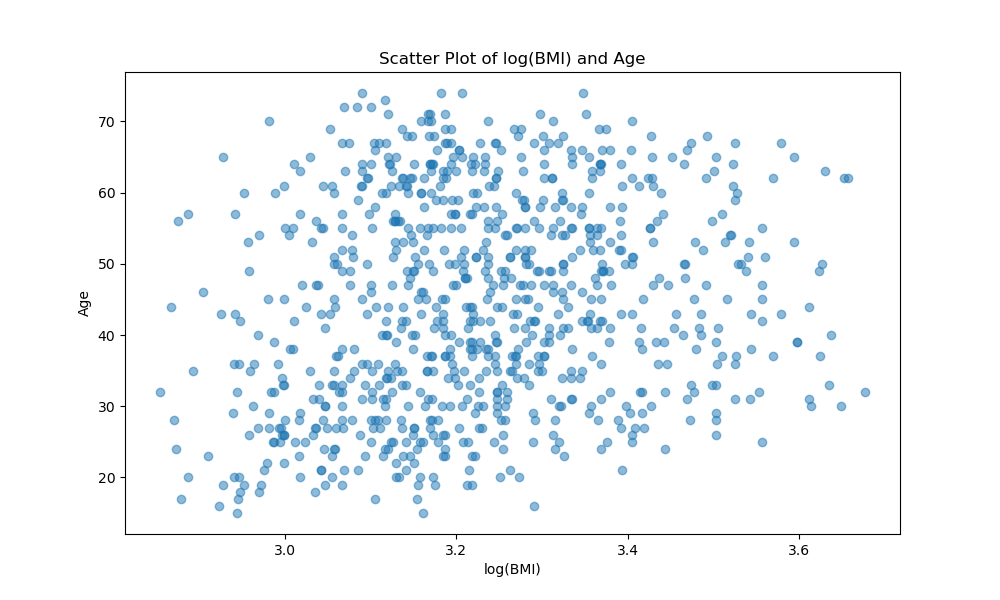
\includegraphics[width=0.75\textwidth]{Figures/scatter_plot_1.png}  % Set width to 75% of text width
    \caption{\small Scatterplot of log(BMI) and Age.}  % Use smaller font for the caption
    \label{fig:scatterplot_1}
\end{figure}
\noindent
\noindent
The same thing can be seen on the scatterplot of the log(BMI) and fastfood where it does not seem there is a correlation between BMI and fastfood, since the data is scattered. 

\begin{figure}[H]
    \centering
    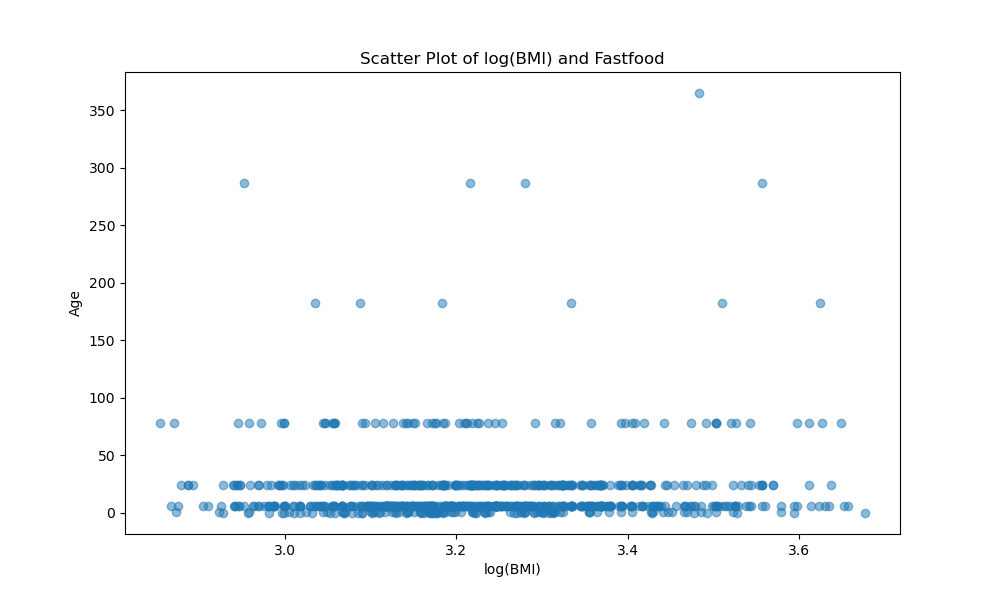
\includegraphics[width=0.75\textwidth]{Figures/scatter_plot_2.png}  % Set width to 75% of text width
    \caption{\small Scatterplot of log(BMI) and Fastfood.}  % Use smaller font for the caption
    \label{fig:scatterplot_1}
\end{figure}
\noindent
\noindent
Further, we undertake a graphical examination of each variable using histograms and box plots. 

\begin{figure}[H]
    \centering
    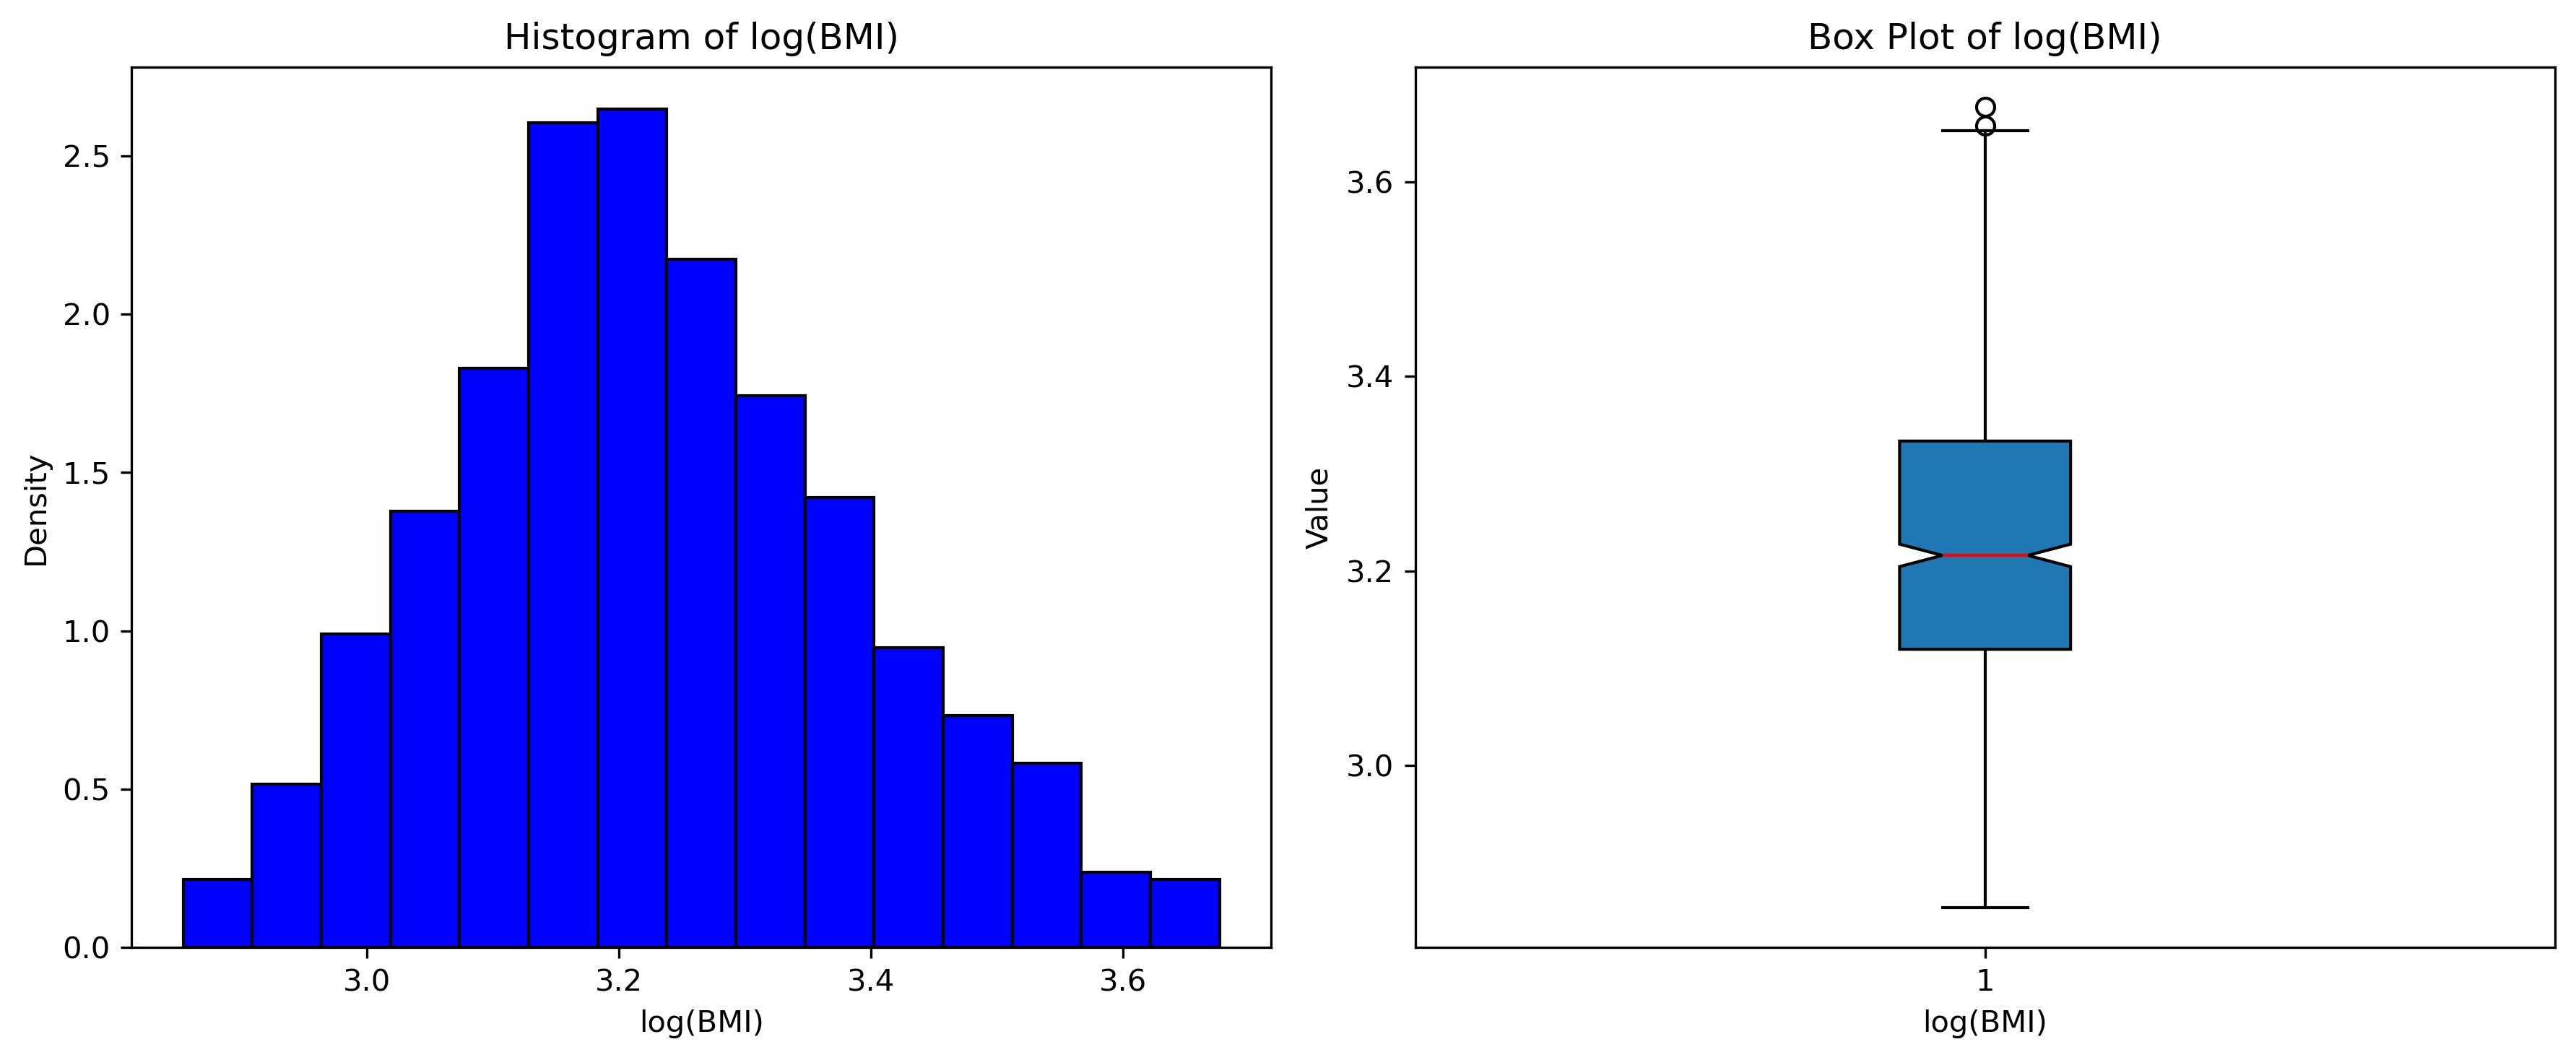
\includegraphics[width=0.75\textwidth]{logbmi_hist_box.png}
    \caption{\small Histogram and boxplot of log(BMI).}
    \label{fig:logbmi}
\end{figure}
\noindent
The histogram for log(BMI) indicates a tendency towards a normal distribution with some skewness. The boxplot highlights a median slightly above 3.2, suggesting a slight skew towards lower values. Notably, a couple of outliers are present on the upper end, indicating some deviations from a typical normal distribution.


\begin{figure}[H]
    \centering
    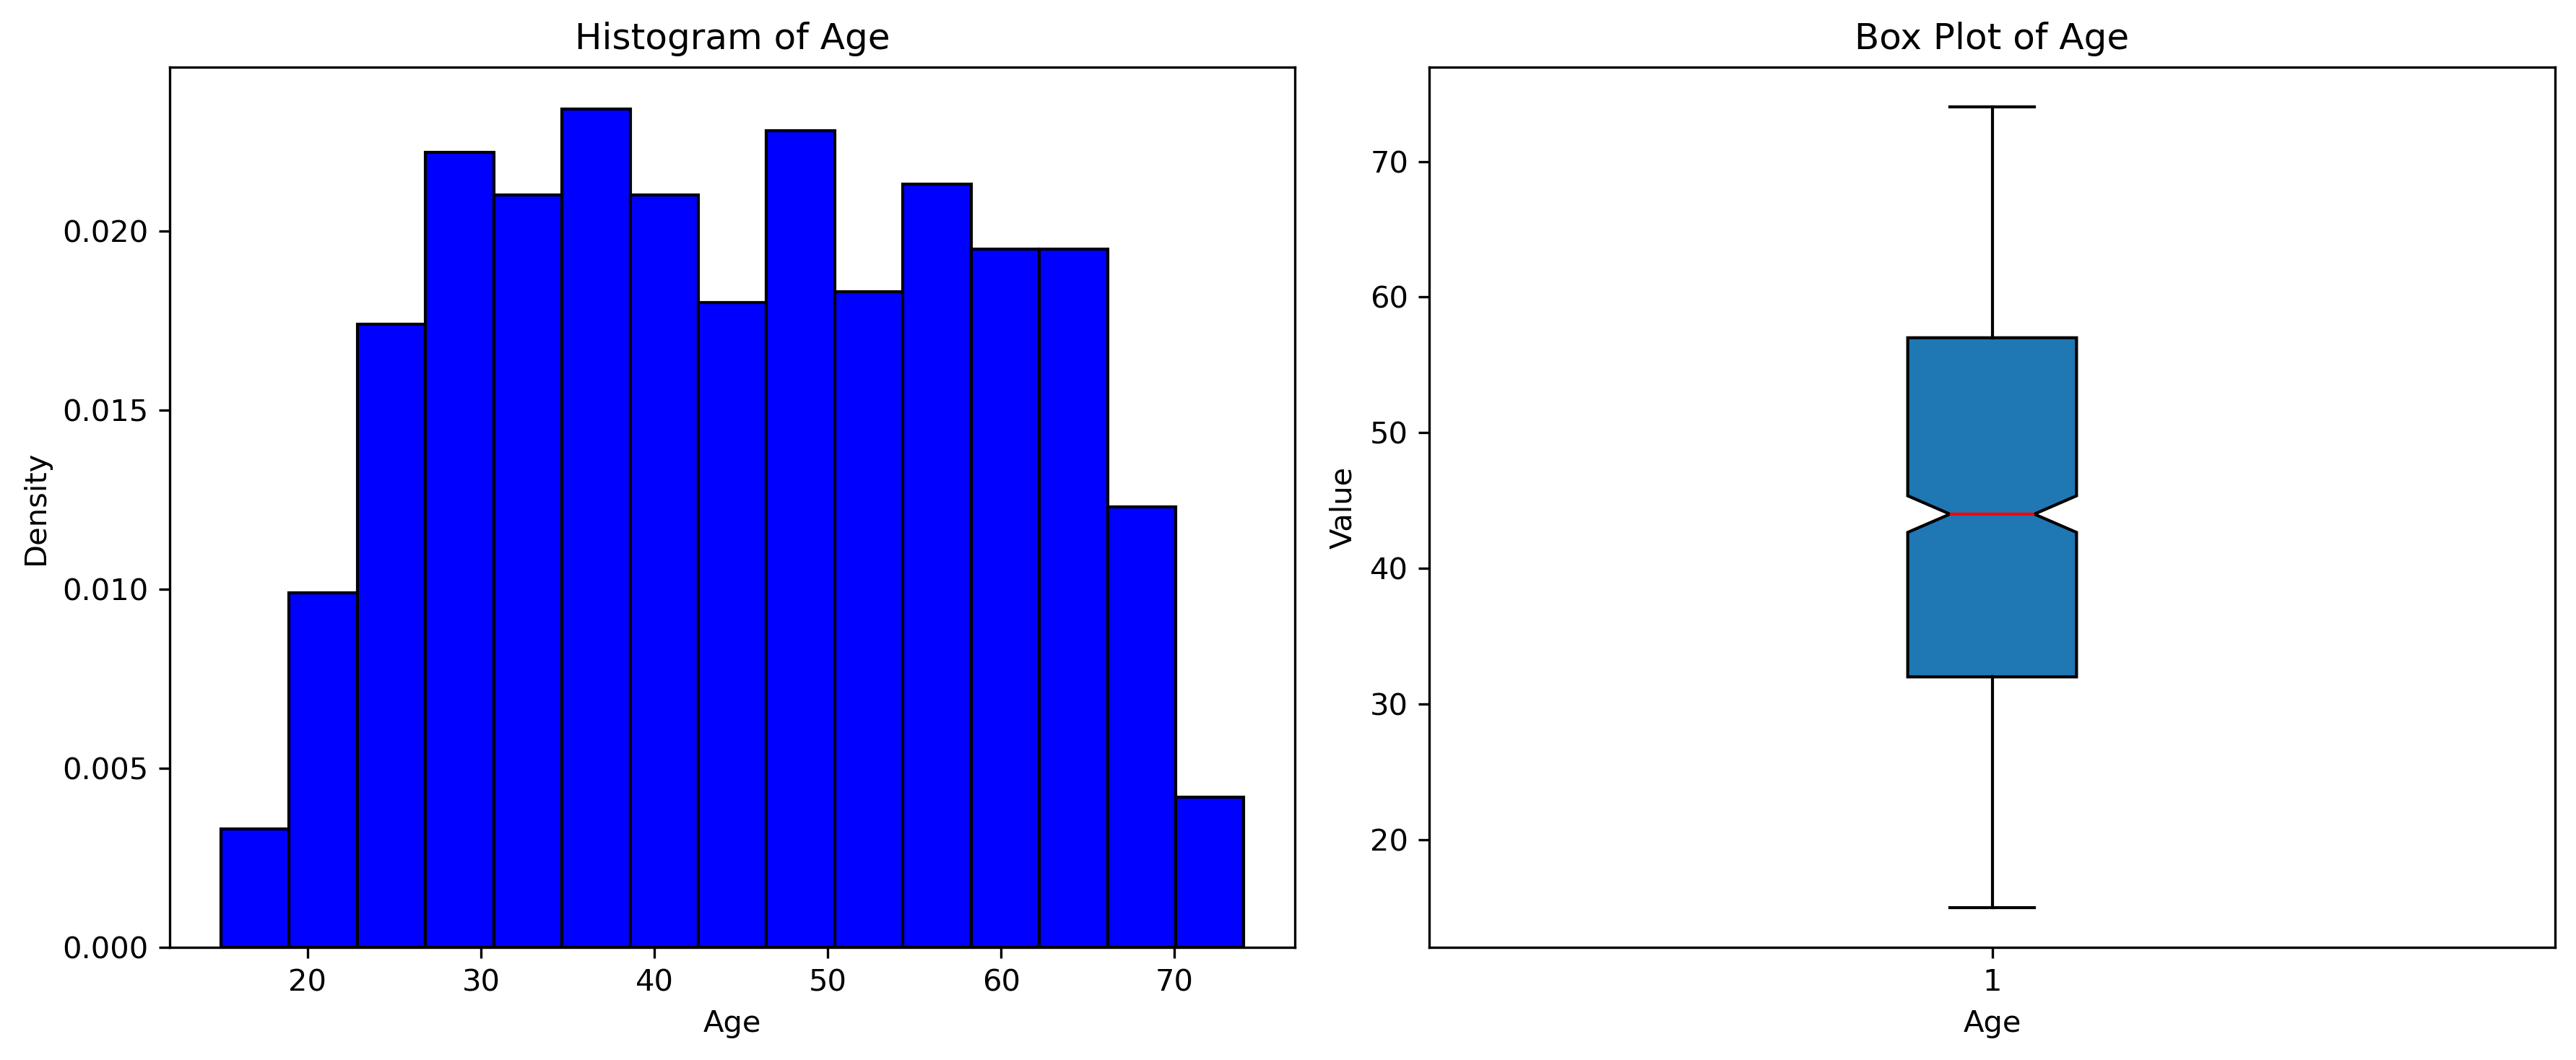
\includegraphics[width=0.75\textwidth]{age_hist_box.png}
    \caption{\small Histogram and boxplot of Age.}
    \label{fig:age}
\end{figure}
\noindent
The histogram for age reveals a broad spread of values, indicative of high variability within the age data. The boxplot shows a median value around 45, nicely centered between the quartiles, reflecting a balanced distribution despite the wide range. The plot suggests a fairly symmetric distribution of age, although the range suggests varied participant ages.


\begin{figure}[H]
    \centering
    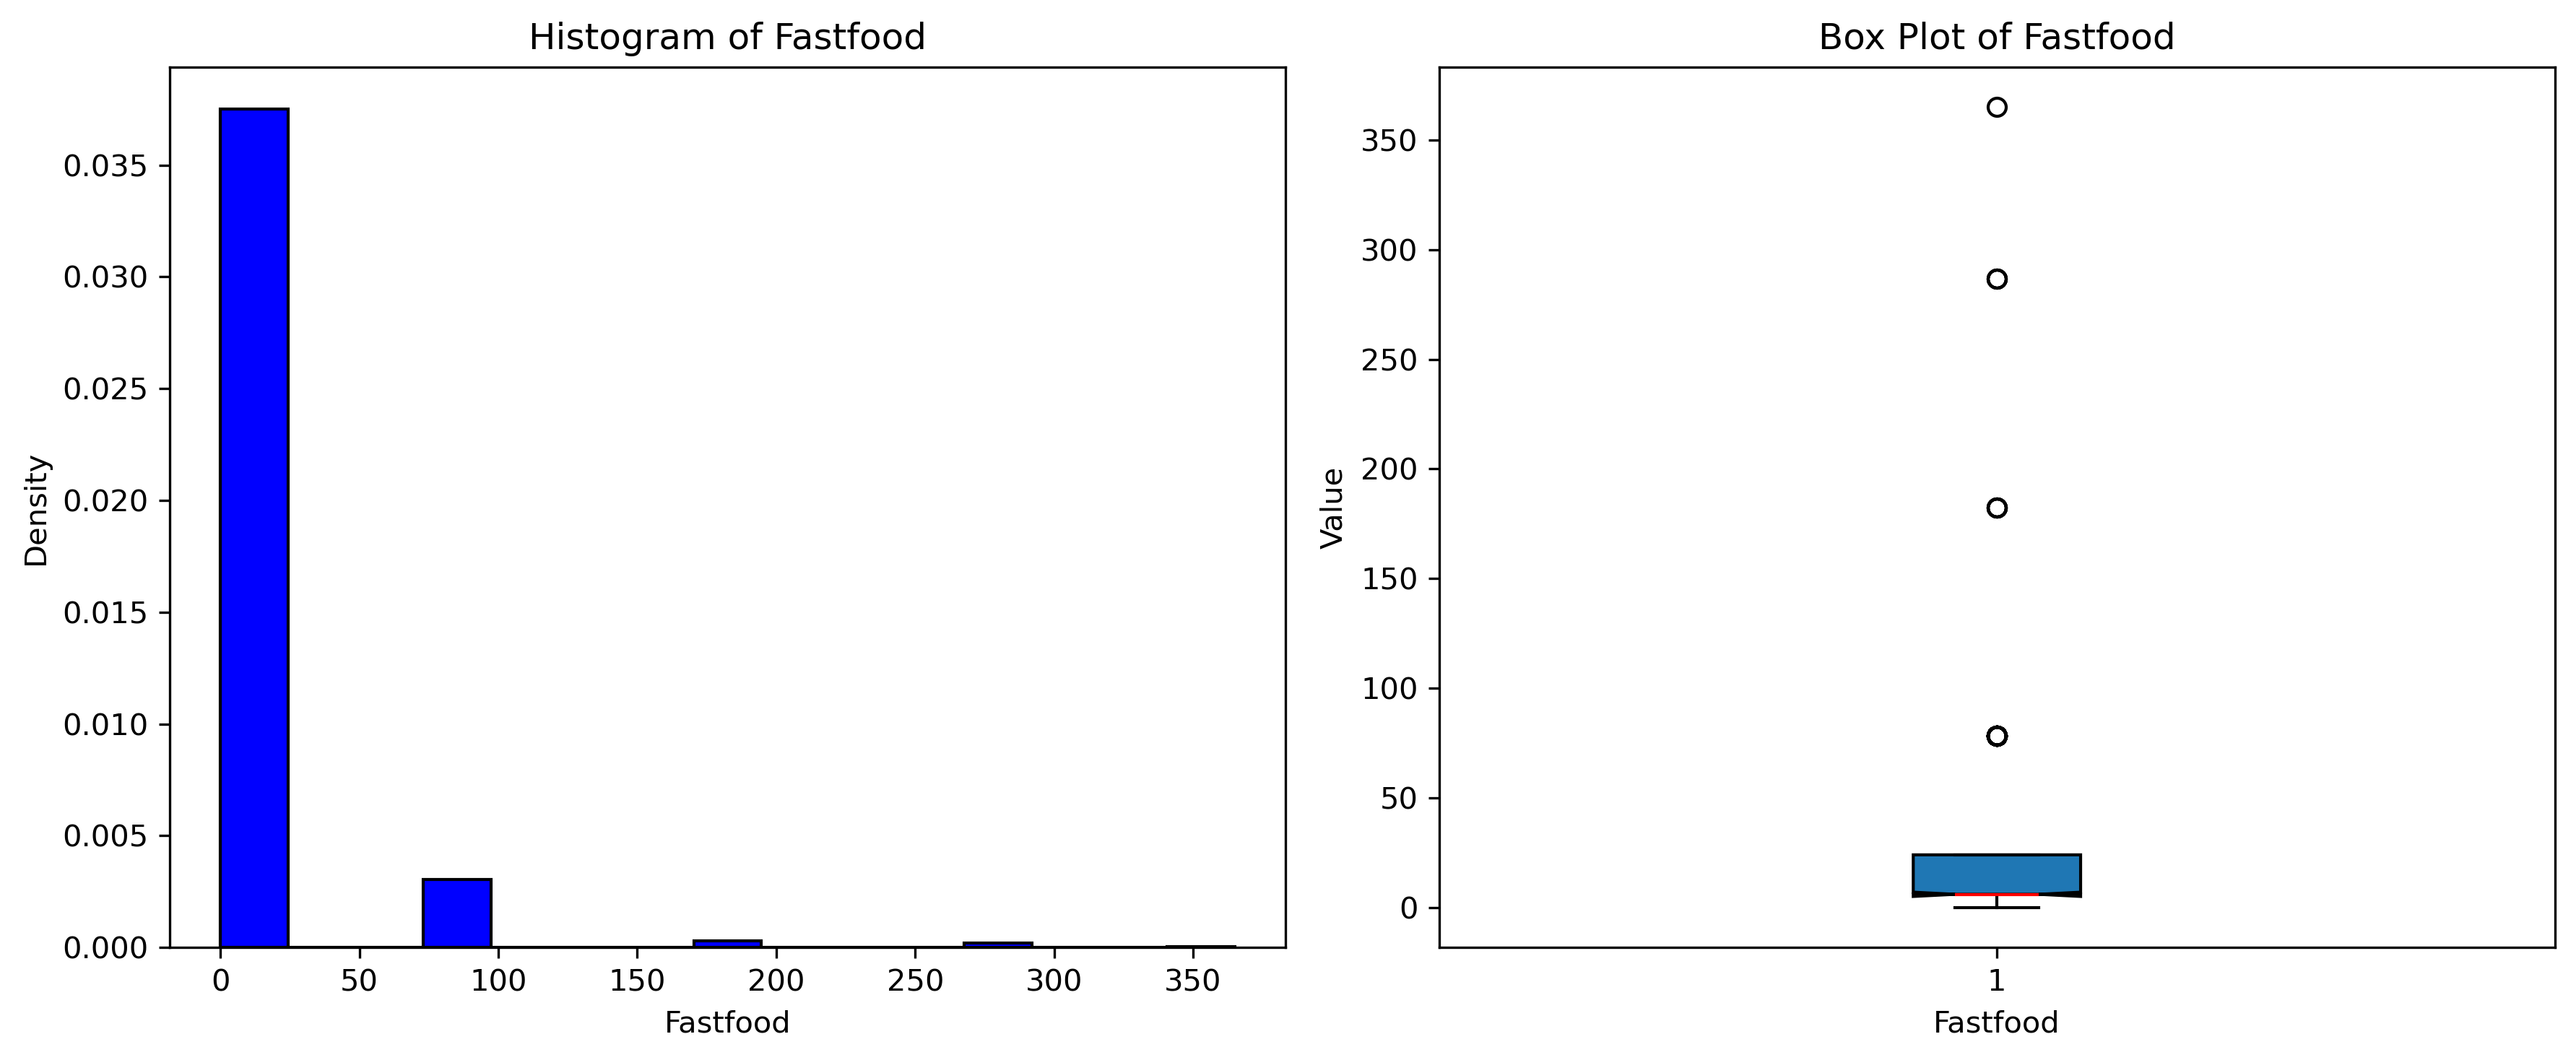
\includegraphics[width=0.75\textwidth]{fastfood_hist_box.png}
    \caption{\small Histogram and boxplot of Fastfood.}
    \label{fig:fastfood}
\end{figure}
\noindent
The fastfood consumption histogram clearly shows a concentration of data points below 100 days, with rare occurrences extending beyond this range. The corresponding boxplot underscores this concentration, with the bulk of data points situated at lower consumption levels. The median, close to the lower quartile, and several high-range outliers highlight the uneven distribution across the dataset.

All relevant data can be seen here:
\begin{figure}[H]
    \centering
    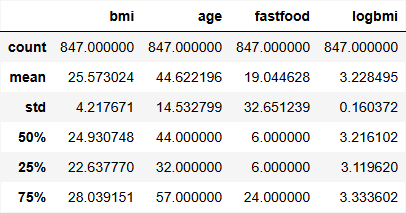
\includegraphics[width=0.8\textwidth]{summary_statistics.png}
    \caption{\small Summary statistics for the dataset.}
    \label{fig:summary_statistics}
\end{figure}

\noindent
The table in Figuredisplays the summary statistics of our main variables. These statistics provide essential insights into the distribution characteristics of each variable, including their central tendencies and variabilities. The median values, along with the first and third quartiles, are particularly helpful in understanding the asymmetry and potential outliers in the data. This detailed statistical overview aids in ensuring the robustness and reliability of subsequent analyses.





\addcontentsline{toc}{subsubsection}{\textbf{b)} Density histogram of the weekly returns from the ETF AGG}
\subsubsection*{\textbf{b)} Density histogram of the weekly returns from the ETF AGG}
\noindent


\addcontentsline{toc}{subsubsection}{\textbf{c)} The weekly return over time for each of the four ETFs}
\subsubsection*{\textbf{c)} The weekly return over time for each of the four ETFs}




\addcontentsline{toc}{subsubsection}{\textbf{d)} Box plot of the weekly returns by ETF}
\subsubsection*{\textbf{d)} Box plot of the weekly returns by ETF}


\addcontentsline{toc}{subsubsection}{\textbf{e)} Summary sizes for the four ETFs}
\subsubsection*{\textbf{e)} Summary sizes for the four ETFs}





\pagebreak
\section{Statistical analysis}
\addcontentsline{toc}{subsubsection}{\textbf{f)} Statistical models describing the weekly return for each of the
four ETFs}
\subsubsection*{\textbf{f)} Statistical models describing the weekly return for each of the
four ETFs}



\addcontentsline{toc}{subsubsection}{\textbf{g)} Confidence intervals}
\subsubsection*{\textbf{g)} Confidence intervals}
\noindent

\addcontentsline{toc}{subsubsection}{\textbf{h)} Hypothesis test}
\subsubsection*{\textbf{h)} Hypothesis test}


\addcontentsline{toc}{subsubsection}{\textbf{i)} Hypothesis Test: Comparison of Weekly Returns from VAW and AGG}
\subsubsection*{\textbf{i)} Hypothesis Test: Comparison of Weekly Returns from VAW and AGG}
\noindent

\addcontentsline{toc}{subsubsection}{\textbf{j)} The importance of statistical test}
\subsubsection*{\textbf{j)} The importance of statistical test}


\addcontentsline{toc}{subsubsection}{\textbf{k)} Correlation between ETFs}
\subsubsection*{\textbf{k)} Correlation between ETFs}


\end{document}
